\chapter{Magnetometer Operation\label{ch:characterization}}

In this Chapter I describe the different ways in which the
magnetometer was operated.  Some of these modes of operation were
applied to furhter experiments, which are reported in
Chapter~\ref{ch:results}.  Some of the modes were simply used to
perform a basic characterization of the magnetometer and to compare
with the results of other groups which were discussed in the
Literature Review in Chapter~\ref{ch:magnetometry}.

The main purpose of this Chapter is to give an overview of the many
parameters which can affect the performance of the magnetometer.
Chapter~\ref{ch:results} goes into further detail on studies of
specific performance metrics under modification of additional
parameters.

The main operation modes of the magnetometer reported in this Chapter
are:
\begin{itemize}
\item Near-zero-field operation.  In this mode, the magnetic field
  must be swept in order to calibrate the magnetometer.  The dynamic
  range of the magnetometer in this case is $|B_z|\lesssim 0.2$~nT.
\item Amplitude modulated NMOR, which itself was used in two distinct modes:
\begin{itemize}
\item Continuously pumped (a.k.a.~forced oscillation) mode.  In this
  mode, the amplitude of the pump beam was modulated continuously and
  the optical rotation signal was demodulated resonantly at the same
  frequency.
\item Free-induction decay (FID) mode.  In this mode, the amplitude of
  the pump beam is modulated for a time and then switched off.  The
  oscillation frequency of the optical rotation signal is then
  measured non-resonantly.
\end{itemize}
In these modes, the magnetometer was generally operated at 0.2~$\mu$T
or 1.0~$\mu$T, which is of considerably more relevance to the nEDM
experiment.
\end{itemize}
In Chapter~\ref{ch:results}, most of the measurements will relate to
our studies using FID mode.  The exception is that some degaussing
studies will be done near zero field and hence will use that mode.


\section{NMOR near zero field and degaussing studies}

During this measurement the pump beam was switched off and the probe
beam is used as its own pump (see
Section~\ref{sec:something-in-chapter-3}).

I used the magnetometer in this mode to study the function of the
degaussing system described in
Section~\ref{sec:Degaussing}.

The experiment was carried out as follows:
\begin{enumerate}
\item The laser beam was tuned for maximum optical rotation and
  stabilized using the DAVLL system.  The beam power was $\sim
  20~\mu$W.
\item Optical rotation of the probe beam was monitored throughout the
  experiment via an oscilloscope monitoring the differential
  photodiode signal.
\item The innermost magnetic shield was degaussed with various
  parameters for the sequence.  The operation of the degaussing
  circuit was described in Section~\ref{sec:Degaussing}.  After
  completing the degaussing sequence a switch is opened to
  electrically isolate the degaussing coil.
\item The magnetic field along the $z$-direction (defined in
  Section~\ref{sec:Internal coil}) is swept in order to calibrate the
  differential photodiode signal as a function of applied $B_z$.  In
  this way the initial magnetic field after degaussing may be deduced.
\end{enumerate}
%In this case,  at first degaussing the shields that surround the vapour cell is done in order to cancel background B-field.A function generator is used to drive the degaussing coil. After completing a degaussing sequence switch is opened to electrically disconnect the degaussing coil from experimental setup. Then B-field ramp is started and NMOR signal is observed through a oscilloscope which  connected to balance photodiode output. The magnetic field sweeping is done in a triangle wave. In 
Fig.~\ref{fig:TUNE} displays the sequence of measurement events in
time, along with the differential photodiode signal (in Volts), which
is proportional to optical rotation.  Also shown is a voltage applied
to the $z$-coil with a 10~k$\Omega$ resistor in series which dominates
the resistance of the circuit.  Recall that the coil constant of the
$z$-coil is $\sim 48$~nT/mA (see Section~\ref{sec:Internal coil}).
The sweep range of this trace is therefore
% (0.8~V)/(10000~Ohm)/*48~nT/mA = 3.84 nT ???  It would be good to
% write the correct calibration constant in the part of the thesis
% where this coil is describe (probably somewhere in Chapter 3).
1.9~nT peak to peak.

In the first section of the oscilloscope trace, the impact of the
degaussing procedure inducing noise in the optical rotation signal can
be seen.  The next section involves the ramping down of a variable
resistor, followed by opening the switch to isolate the degaussing
coil.  Then the magnetic field $B_z$ is swept and the characteristic
dispersive Lorentzian shape of NMOR is observed.

\begin{figure}%[h]
\centering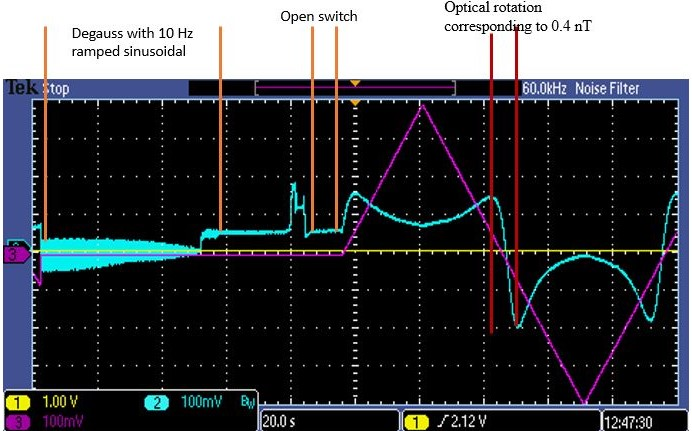
\includegraphics[width=0.7\linewidth]{figures/scope_trace_of_field_sweeping}
\caption{Oscilloscope trace of measurement OR near zero field. The
  purple curve shows the voltage across the 10~k$\Omega$ resistor in
  series with the $z$-coil, from which the magnetic field ramp of
  1.9~nT peak to peak can be deduced.  The blue trace indicates the
  differential photodiode signal which is proportional to the optical
  rotation.  The left side of the traces show the impact of the
  degaussing procedure, while the right side shows the calibration
  procedure.\label{fig:TUNE} }
\end{figure}


In this measurement NMOR signal is used to determine effectiveness of
degaussing procedure. After the degaussing procedure the observed OR
signal is non-zero while the applied field $B_z$ was zero which
indicates the existence of a remnant field.  The effect of degaussing
parameters sensed by the magnetometer is discussed further in
Section~\ref{sec:degaussing}.


% We need to have this table somewhere, but I think it needs to be in
% the section where you talk about degaussing.

%\begin{table}%[h]
%\centering
%\begin{tabular}{|l|l|}
%\hline
%\textbf{SETTING}    & \textbf{VALUE} \\
%\hline
%Function generator &   \\
%\hline
%Frequency &  10 Hz   \\
%Sample rate    &  10000 sample/sec  \\
%Amplitude   &   10 V \\
%Offset  &       0 V  \\
%\hline
%\end{tabular}
%\caption{Setting for degaussing \label{table:degaussing setting}}
%\end{table}

Fig.~\ref{fig:near zero field} shows an example of the calibration of
the differential photodiode signal to the field applied by the
$z$-coil, for data where the degaussing part of the sequence have been
removed.  The field is calibrated to the voltage signal as described
above.  In Fig.~\ref{fig:near zero field}, the data have been fitted
to a dispersive Lorentzian shape given by the function
\begin{equation}
\mathrm{Signal~(V)}=\frac{a(B-B_0)}{1+a(B-B_0)^2}\cdot l+C
\end{equation}
where $a$, $B_0$, $C$, and $l$ are fit parameters.  A key measure of
magnetometer performance is the valley-to-peak distance, which in this
case is about $\Delta B=\frac{2}{a}=0.49$~nT.  The other key measure
in this case is the deduced field at zero crossing given by the fit
parameter $B_0=0.019$~nT.  Thus, after degaussing, a remanent field of
19~pT is found.  This is only the on-axis field.  It is possible that
transverse fields can be larger, and these tend to make the width
$\Delta B$ of the zero-field curve larger.

\begin{figure}[h]
\centering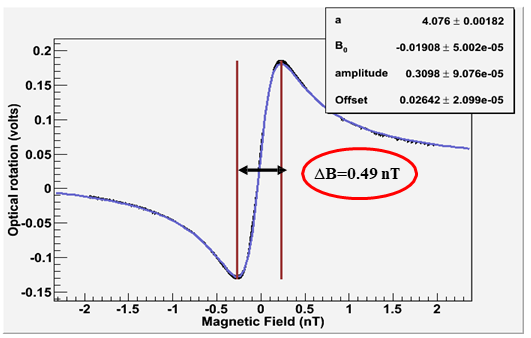
\includegraphics[width=0.7\linewidth]{figures/near_zero_field}
\caption{Optical rotation as a function of magnetic field applied
  along the direction of the laser beam. The signal looks like a pure
  dispersive Lorentzian curve. The measured resonance width is 0.49~nT
  and the measured remanent field is 0.019~nT.\label{fig:near zero
    field}}
\end{figure}

In order to determine the sensitivity, a magnetometer can be operated
in different modes. Most of them found its application during the time
this Master's thesis was prepared. Although main focus of this work
was to study magnetometer performance in Free Induction Decay (FID)
mode.

\section{Amplitude Modulated NMOR:  Forced-Oscillation Mode}

In forced-oscillation measurement mode, the pump beam amplitude is
modulated and the differential photodiode signal is demodulated at the
same frequency $\Omega_m$ using a lock-in amplifier.  The
modulation/demodulation frequency is near twice the Larmor frequency
of the atoms in the magnetic field.

%In the first instance, we tried keeping the frequency constant and
%sweeping the magnetic field.  We can then determine the resonant field
%by fitting the resonance lineshape.  The disadvantage of this method
%is that the field must be changed in order to measure it.

%{\bf An
%  example of this might be shown in Fig.~\ref{fig:AMORmaybeidontknow},
%  or it might not be.  Really, it is impossible to tell.}

%\begin{figure}[h]
%\centering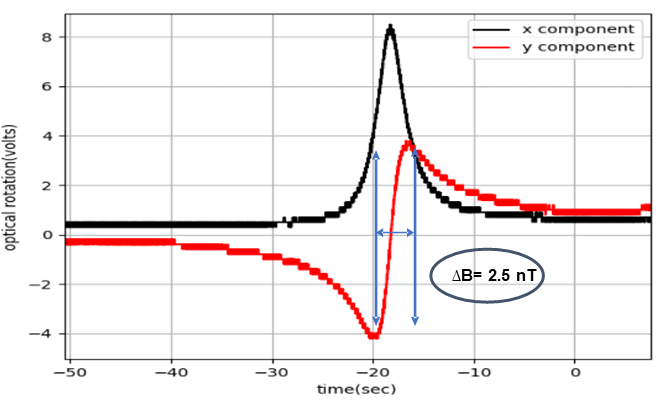
\includegraphics[width=0.7\linewidth]{figures/AM_NMOR}
%\caption{\bf The rest of this figure caption might be totally
%  false... AMOR resonance signal with a 5 cm cell containing natural
%  Rb.  Data was acquired by using a balanced photodiode which
%  demodulated through lock-in amplifier as the frequency is swept
%  slowly near 9.37~kHz.  The parameters of the sweep are shown in
%  Table~\ref{tab:freqsweep} and are discussed further in the text. The
%  observed resonance width, when translated from frequency into field,
%  is 2.5~nT.\label{fig:AMORmaybeidontknow}}
%\end{figure} 

%A better way to measure the field without having to change it is to
%sweep the modulation/demodulation frequency instead.  The resonant
%frequency then gives a determination of the field (when
%$\Omega_m=2\Omega_L$)

%\begin{figure}[h]
%\centering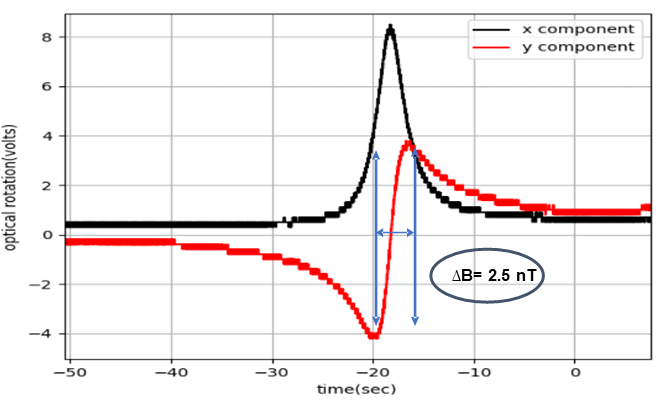
\includegraphics[width=0.7\linewidth]{figures/AM_NMOR}
%\caption{\bf I do not know what this figure is, and so here is what
%  I'm guessing that it might be: AMOR resonance signal with a 5 cm
%  cell containing natural Rb.  Data was acquired by using a balanced
%  photodiode which demodulated through lock-in amplifier as the
%  frequency is swept slowly near 9.37~kHz.  The parameters of the
%  sweep are shown in Table~\ref{tab:freqsweep} and are discussed
%  further in the text. The observed resonance width, when translated
%  from frequency into field, is 2.5~nT.\label{fig:AMOR}}
%\end{figure} 

%Fig.~\ref{fig:AMOR} {\bf potentially, maybe, and if it doesn't we
%  should find the figure that does show this, since you included the
%  table below which relates to the data that may or may not be
%  presented in the figure but should be} shows a measurement of the
%in-phase and quadrature signals measured while the frequency is swept
%very slowly.  The parameters of this mode of operation, particularly
%of the slow frequency modulation, are shown in
%Table~\ref{tab:freqsweep}.

%\begin{table}%[h]
%\centering
%\begin{tabular}{|l |l|}
%\hline
%
%\textbf{ SETTING}    & \textbf{VALUE} \\
%\hline
%Function generator &   \\
%\hline
%Frequency & 9.37kHz   \\
%
%Waveform    &  Square  \\
%
%Amplitude   &  $1V_{pp}$  \\
%Offset  &       500 mV  \\
%Duty cycle       &    $1\%$ \\
%Frequency Deviation     &   40 Hz  \\
%FM Frequency     &   100 mHz  \\
%modulation waveform      &    Triangle \\
%Amplitude modulation & On \\
%\hline
%Lock-in amplifier &     \\
%\hline
%Lock in frequency     & 9.37 KHz \\
%Time constant     &  $300\mu s$ \\
%Sensitivity      &  100mV  \\
%\hline
%\end{tabular}
%\caption{Setting for AM NMOR at $1\mu$T field {\bf which may or may
%    not correspond to any other data showed in any other figure of
%    these thesis.  All other parameters of the measurement are
%    apparently unknown.}.\label{tab:freqsweep}}
%\end{table}

%Fig.~\ref{fig:AMOR} shows the characteristic dispersive and absorptive
%shapes in the in-phase and quadrature signals, respectively.  This is
%in good agreement with expectation.  The quality of the magnetometer
%is again characterized by the peak-to-valley distance in frequency,
%which, when translated to field corresponds to a width of 2.5~nT.

%A drawback of this mode of operation is that the drive frequency is
%constantly changing, so that each data point for optical rotation
%represents a range of drive frequencies that were sampled within the
%lock-in time constant.  A more robust method involves selecting
%particular frequencies in series and then fitting to determine the
%resonant frequency, as done in Ref.~\cite{mythesis}.  I tried
%this method also, which I call a forced-oscillation scan.

For a forced-oscillation scan, a frequency range and frequency
increments are entered into a custom Python code. Via a USB
connection, the function generator driving the AOM is set to the
appropriate frequencies in sequence.  This thereby changes frequency
of modulation $\Omega_m$ of the pump beam in the magnetometer.  The
reference signal of the function generator is used as the reference
signal for the lock-in amplifier.  The differential phototdiode output
is demodulated at the reference frequency. The resulting in-phase (X)
and quadrature (Y) outputs are collected from the lock-in amplifier by
the Python code via GPIB.  A settling time of at least 5 lock-in time
constants ensures that no memory of the previous frequency is retained
by the lock-in amplifier.


\begin{figure}%[h]
\centering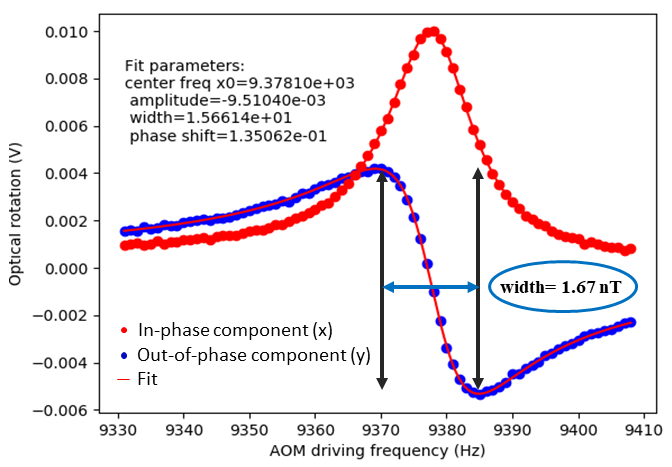
\includegraphics[width=0.5\linewidth]{figures/FM_modulation}
\caption{Demodulated components of the differential photodiode signal,
  as a function of the forced-oscillation frequency.  The red points
  indicate the demodulated X output.  The blue points indicate the Y
  output.  The data are fitted using the fit function described in the
  text in order to determine the resonant frequency.  The results of
  the fit are shown in the red curve drawn through both the X and Y
  points.  The fit parameters for this fit are shown in the legend of
  the graph and are discussed further in the text.  The vertical lines
  indicate the peak-to-valley distance in frequency, and are
  translated into a magnetic field width of 1.67~nT using the
  gyromagnetic ratio.\label{fig:FMOR}}
\end{figure} 


Fig.~\ref{fig:FMOR} shows an example of the resultant X (red) and Y
(blue) outputs for the various $\Omega_m$ settings.  The range of
drive frequencies used in Fig.~\ref{fig:FMOR} was 9.31 kHz to 9.409
kHz, corresponding to an applied magnetic field of $\sim 1~\mu$T
directed along light propagation direction.  The pump beam was
modulated with a square wave with duty cycle 1\%.  The small duty
cycle is used to reduce the influence of the pump beam on the probe
measurement.

As can be seen in Fig.~\ref{fig:FMOR}, the X output reaches a maximum
and the Y output crosses zero near $\Omega_m=2\Omega_L$.  The data are
fitted in order to determine the resonant frequency and other
parameters.

The functions being fitted simultaneously are~\cite{mythesis}:
\begin{equation}
\phi_Y=\frac{A_0 (f-f_0 )\Delta f}{2(f-f_0 )^2+(\Delta f)^2/4}\cos\theta-\frac{(\Delta f)^2A_0}{(f-f_0 )^2+(\Delta f)^2/4}\sin\theta+C
\end{equation}
and
\begin{equation}
\phi_X=\frac{A_0 (f-f_0 )\Delta f}{2(f-f_0 )^2+(\Delta f)^2/4}\sin\theta+\frac{(\Delta f)^2A_0}{(f-f_0 )^2+(\Delta f)^2/4}\cos\theta+D.
\end{equation}
Here, $\phi_{X,Y}$ represent the lock-in amplifier outputs, which are
measured as a function of frequency $f$.  The fit parameters are:
$A_0$, which represents the maximum of the purely absorptive curve;
$\Delta f$, the width of resonance (FWHM); $f_0$ the central resonance
frequency; a phase shift $\theta$; and offsets C and D.

For the fit presented in Fig.~\ref{fig:FMOR}, the fit parameters are
$A_0=-0.0095$~V, $f_0=9378.1$~Hz, $\Delta f=15.7$~Hz,
$\theta=0.135$~radians.  The small phase shift $\theta$ is likely
induced by the finite duty cycle of the pump beam, and small time
delays in the system.  The offsets $C$ and $D$ are small, and are
likely induced by small voltage offsets in the oscilloscope or lock-in
outputs (which can be re-zeroed freely).

%The overall fitting function in order to really fit a
%complex Lorentzian is given by (the phases in R(x) and D(x) are not
%considered in the following equations, since they are varied
%(sin/cos)).


A techical detail of the simultaneous fitting process is that the
$\phi_X$ and $\phi_Y$ data are catenated into a single array of
values, which are then fitted in different regions using the two
different functions above, in a single overall least-squares fit.  The
process is similar to that described in Ref.~\cite{mythesis}.

Based on this measurement, the magnetic field is 1.004635 $\mu$T which
is translated from central frequency $f_0= 9.37810$ kHz. The width
$\Delta f=15.66$~Hz is important, because the narrower the width, the
more precise the measurement of the magnetic field would be.  The
width can also be translated into magnetic field using the relation
$\Delta B= \Delta f/2 \gamma$ where $\gamma$ is the gyromagnetic ratio
of Rb as discussed in Section~\ref{sec:Rb structure}.  This results in
a value of 1.67~nT for the width.

In general, measurements of the magnetic field that are a factor of a
thousand more precise than the width are possible in forced
oscillation mode.  As discussed in Chapter 2, in Ref.~\cite{mythesis},
a statistical precision of about 0.17~pT was achieved in scans of this
form.  Rather than fully optimizing this method, we decided instead to
focus on the free-induction decay mode of operation, described in the
next section.


% Probably these points should be discussed in the Literature Review
% in relation to Michi's thesis.

%Advantages: In the force oscillation scan technique entire resonance curve is scanned which allow us to see if there is a pure resonance or the real resonance curve get destroyed by any other external influences. By mapping out the entire resonance curve, we can easily debug the problem because in this process we can repeatedly adjust the power of the pump and probe beam immediately after each scan. Since the output signal of the balanced photodiode is demodulated stepwise by the lock-in amplifier at the modulation frequency at each increment, small amounts of noise induce in this process which is the most advantageous point of this field measurement technique. \\

%Disadvantages: The force oscillation scan is a quite slow process which is the main drawback of this measurement scheme.

%For a scan range of some hundred Hz usually takes a few minutes with  waiting time of couple second. As a result the force oscillation scans are not directly sensitive to magnetic field drifts, occurring at time intervals which are shorter than the actual scan. Field drifts would cause a degradation of the precision of a swept oscillation scan.

%\subsection{Self oscillation mode}

% This should be in Chapter 2.




\subsection{Free Induction Decay}

The focus of this thesis was to study the magnetometer operation in
free induction decay (FID) mode.  In FID mode, the quantum state of
the Rb atoms inside the cell is prepared using the pump beam, and then
the pump beam is switched off and the precession frequency of the
coherent state is measured using the probe beam.  The measured
precession frequency then determines the field via the gyromagnetic
ratio.

Fig.~\ref{fig:FID_example} shows an example of a pump/probe
measurement cycle in FID mode at a field of $\sim 0.2~\mu$T.  The
signal in the differential photodiode output is seen to grow when the
AM pump beam is switched on.  After the pump is switched off, the
collection of the FID signal begins.  The differential photodiode
signal continues to oscillate and decays away exponentially in time.
The measurement of the oscillation frequency of the probe beam in the
FID signal region gives the magnetic field.

\begin{figure}%[h]
\centering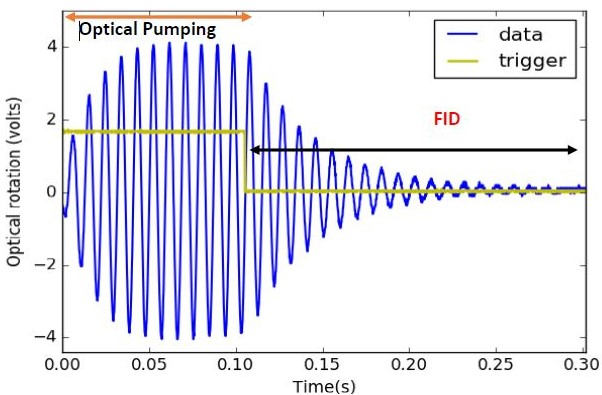
\includegraphics[width=0.55\linewidth]{figures/Capture2}
\caption{Sample FID measurement cycle.  The curve labelled ``data''
  (blue) indicates the differential photodiode signal, as demodulated
  in the lock-in amplifier.  Only the X (in-phase) signal is shown.
  The curve labelled ``trigger'' is a signal which indicates a
  non-zero value when the pump beam is on and with the amplitude
  modulation described in the text.  The pump phase is indicated by
  the orange arrow ``Optical Pumping'' which persisted for times from
  0.0~s to 0.1~s.  The probe phase is indicated by the black arrow
  ``FID'' which was done for the subsequent 0.2~s. The applied
  magnetic field during the measurement is
  $0.2~\mu$T.\label{fig:FID_example}}
\end{figure}

In Fig.~\ref{fig:FID_example}, the differential photodiode signal has
been demodulated using a lock-in amplifier whose frequency has
purposely been set to be about 100~Hz away from the oscillation
frequency of the atoms.

Table~\ref{tab:FID_setting} shows the function generator (fed to the
AOM driver) and lock-in amplifier settings for FID measurement at
$0.2~\mu$T.

\begin{table}[h]
\centering
\begin{tabular}{|l |l|}
\hline

\textbf{ SETTING}    & \textbf{VALUE} \\
\hline
Function generator &   \\
\hline
Frequency & 2.034 kHz   \\

Waveform    &  Square  \\

Amplitude   &  $1V_{pp}$  \\
Offset  &       500 mV  \\
Phase       &    $0\degree$ \\
Trigger     &   Manual  \\
Burst       &    220 cycle \\
Amplitude modulation & On \\
\hline
Lock-in amplifier &     \\
\hline
Lock in frequency     & 1.9439 KHz \\
Time constant     &  $300\mu s$ \\
Sensitivity      &  500mV  \\
\hline
\end{tabular}
\caption{Setting for FID at $0.2~\mu$T field.\label{tab:FID_setting}}
\end{table}

The amplitude of the pump beam is again modulated at $\Omega_m\approx
2\Omega_L$, using again a square-wave with low duty cycle.  Generally,
the oscillation frequency is adjusted initially to maximize the
initial amplitude of the FID once the pump beam has been switched off.

The reference signal on the lock-in amplifier has further to be set
slightly off resonance ($\sim 100$~Hz) in internal frequency mode.
The frequency offset may be adjusted in order to enhance the number of
zero crossing of the FID signal and hence get a better measurement of
the beat frequency.  In Section~\ref{sec:lockinoffset} I study the
impact of this setting further.

The X and Y outputs of the lock-in amplifier are recorded using a
Tektronix oscilloscope.  A Python script may be used to transfer the
data from the oscilloscope to computer for further analysis.

In Fig.~\ref{fig:FID_example}, the FID signal recorded by the X
channel is sinusoidal with an exponentially decaying envelope, and may
be fitted in order to determine the beat frequency
\begin{equation}
X(t)=X_0+Ae^{-(t-t_0)/\tau}\sin(\omega
t+\phi_0).\label{eq:decaying_sinwave}
\end{equation}  
To gain in precision, the signal from the Y channel is also recorded
and may be simultaneously fit to a decaying cosine wave:
\begin{equation}
Y(t)=T_0+Ae^{-(t-t_0)/\tau}\cos(\omega
t+\phi_0).\label{eq:decaying_coswave}
\end{equation}
where $y_0$ describes a possible offset, A is the maximum amplitude of the sinusoidal oscillation,
t the present time, $t_0$ the starting point of the measurement, $\omega$ the oscillation frequency and $\phi_0$  some possible phase shift. The data fitting procedure were done in two ways in order to study a variety of systematic effects that were encountered. One method is to take a least square fit of x and y data separately to a decaying sin and cosine wave respectively. Another way of data fitting is to fit x and y data simultaneously. A least square-fit of the recorded data set to equation \ref{eq:decaying_sinwave} and \ref{eq:decaying_coswave} gives an estimate on frequency and  therefore the magnetic field.
\begin{figure}[h]
\centering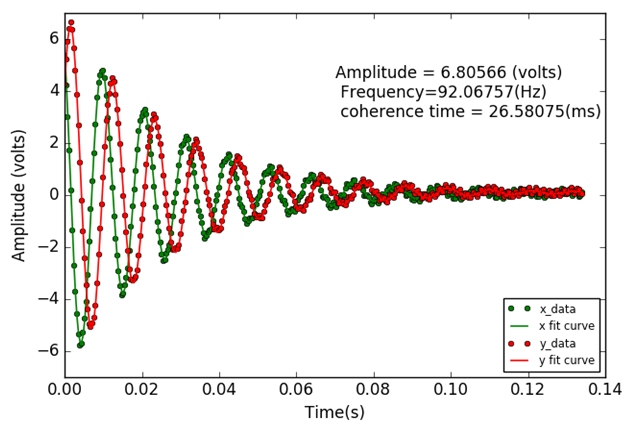
\includegraphics[width=0.55\linewidth]{figures/fid_simultaneous}
\caption{ Simultaneous fit of X and Y signal (green and red dots are represents x and y data respectively whereas green and red line  represents fit curves\label{Fig:FID fit}}
\end{figure}
  

The initial guesses for the least-square parameters are given
as:
\begin{itemize}
\item
Beat frequency $\omega$: In order to guess the beat frequency, the Fast Fourier Transform (FFT) of FID signal is done. The extracted FFT frequency is used as guess frequency.
\item
Amplitude A: In order to get guess amplitude, Averaging the maximum of the X and Y data is done.
\item
Offset $\phi_0$: The mean of FID signal is calculated. This mean value is used as guess for the offset. 

\end{itemize}
The data fitting procedure provides us the actual value for those parameters. The oscillation frequency, one of the extracted fit parameters, is then is used to estimate the magnetic field according to the following equation
\begin{equation}
 B= \frac{\nu_{fit}~ +~\nu_0}{2\gamma}\label{eq:field}
\end{equation}
 where $\nu_{fit}$ denotes the oscilation  frequency, $\nu_{0}$ is lock-in frequency and $\gamma$ is the gyromagnetic ratio of Rb vapor(see section \ref{sec:Rb structure}). Fig \ref{Fig:FID fit} shows an example least square fit of FID signal where both x and y output of lock-in has displayed.
 
Advantages: FID mode is free of  pump light induced frequency shifts or instabilities because the optical pumping is done for a very short time period and the frequency measurement takes place quickly. This frequency is later translate into magnetic field.\\ 

Disadvantages: As a finite duty cycle is used (pump modulation only happens during a short period of time and the main idea is to watch the coherence decay, a decreasing of the maximum achievable sensitivity with this method.



\subsection{FID in tilted magnetic field}
For the nEDM experiment it is very important to do tilted field measurement in order to have better understanding of  geometric phase effects which are the leading sources for systematic uncertainties during nEDM measurement . 
Since our Rb magnetometer is a scalar magnetometer, it is not possible to measure vector field components directly. In this study the NMOR Signal was observed by connecting the balanced photodiode to the oscilloscope directly. A python script is used to transfer the data presented on the oscilloscope screen to computer for further analysis. 

\begin{figure}
    \centering
 
    \begin{subfigure}[b]{0.45\textwidth}
        \centering
        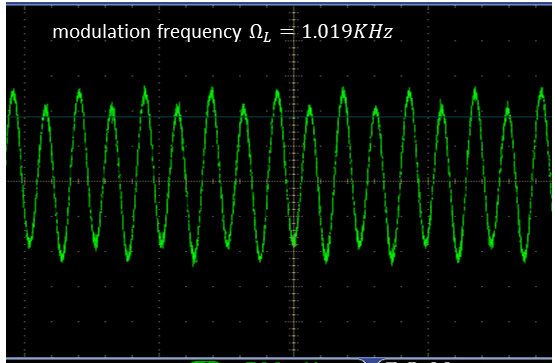
\includegraphics[width=\textwidth]{figures/transverse_field}
        \caption{}
        \label{fig:transverse}
    \end{subfigure}
    \hfill
    \begin{subfigure}[b]{0.45\textwidth}
        \centering
        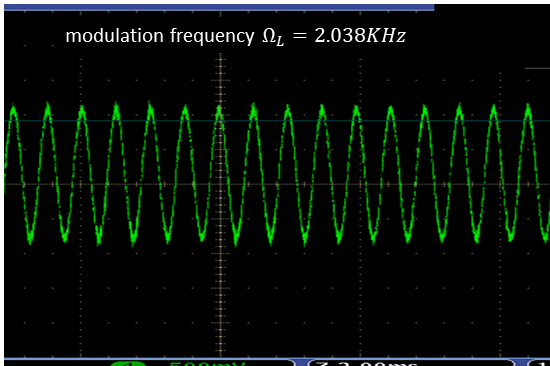
\includegraphics[width=\textwidth]{figures/transverse_field_2}
        \caption{}
        \label{fig:transverse2}
    \end{subfigure}
    \caption{(a) Optical rotation as a function of time at $\Omega_L$ in the yz plane at tilt angle $15\degree$ with light propagation direction. (b) Optical rotation as a function of time at $2\Omega_L$ for same tilt angle}
    \label{fig:Tilted field}
\end{figure}

